\newpage
\section*{Keynote}\addcontentsline{toc}{section}{Keynote}


The keynote address for SMPC 2019, \textit{Fire and Ice: A Case Study for the Sounds of Poetry Viewed as Music}, will be given by Fred Lerdahl, Professor Emeritus at Columbia University, in Loewe Theater at 5:30 PM on August 5th.


\subsection*{Abstract}

The sounds of poetry, like those of music, combine perceptually into hierarchically organized structures, making it possible to treat poetic sounds as if they were music. Using Ray Jackendoff's and my cognitively oriented music theory along with contemporary work in generative phonology, I explore this idea by developing a rule system that assigns to poetic lines the following structures: word groupings, stress and metrical grids, syllable durations, intonation contours, and hierarchical patterns of syllabic repetition and contrast. I illustrate these structures through an analysis of a short poem by Robert Frost, {\it Fire and Ice}. Three audio readings of the poem are compared to the analysis. In addition to providing a systematic method of poetic analysis, this study reveals structural features that poetry and music do and do not share. The talk closes with a presentation of my piece {\it Fire and Ice}, which is based in part on the foregoing poetic analysis and audio readings.

\subsection*{Biography}
\begin{wrapfigure}{r}{0.3\textwidth}
\centering
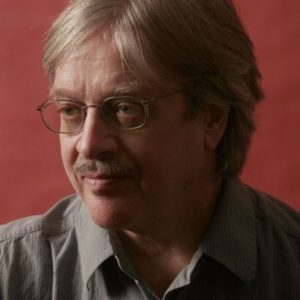
\includegraphics[width=1\linewidth] {images/lerdahl.jpg}
\end{wrapfigure}

Fred Lerdahl's music has been commissioned and performed by major chamber ensembles and orchestras in the United States and around the world, and he has been resident composer at leading institutions and festivals. His music is published by Schott Music Corporation and has been widely recorded for various labels including Bridge Records, which is producing an ongoing series of his music. Lerdahl is a member of the American Academy of Arts and Letters.

His seminal book {\it A Generative Theory of Tonal Music}, co-authored with linguist Ray Jackendoff, is a foundational document in the cognitive science of music. His second book, {\it Tonal Pitch Space}, which extends ideas from the earlier book, won the 2003 distinguished book award from the Society for Music Theory and an ASCAP-Deems Taylor award. A third book, {\it Composition and Cognition: Reflections on Contemporary Music and the Musical Mind}, based on his 2011 Bloch Lectures at UC/Berkeley, brings together his dual activity as composer and theorist; it will be published in November 2019. He has also published many articles in music theory and cognition, including ``Timbral Hierarchies,'' ``Cognitive Constraints on Compositional Systems,'' ``Atonal Prolongational Structure,'' and ``Modeling Tonal Tension'' (co-authored with music psychologist Carol Krumhansl).

Lerdahl studied at Lawrence, Princeton, and Tanglewood. He taught at UC/Berkeley, Harvard, and Michigan, and from 1991 to 2019 he was Fritz Reiner Professor of Musical Composition at Columbia, where he directed the composition program for 20 years.
